% !TEX root = ./main.tex

\documentclass{article}
\usepackage[utf8]{inputenc}
\usepackage[ngerman]{babel}
\usepackage{pdfpages}
\usepackage{graphicx}
\usepackage{amsmath}

\graphicspath{ {./img/} }
\usepackage{hyperref}
\usepackage{lipsum}
\usepackage{float}
\usepackage{listings}

\usepackage{xcolor}

\definecolor{codegreen}{rgb}{0,0.6,0}
\definecolor{codegray}{rgb}{0.5,0.5,0.5}
\definecolor{codepurple}{rgb}{0.58,0,0.82}
\definecolor{backcolour}{rgb}{0.95,0.95,0.92}

\setlength{\parindent}{0pt}

\lstdefinestyle{mystyle}{
    backgroundcolor=\color{backcolour},   
    commentstyle=\color{codegreen},
    keywordstyle=\color{magenta},
    numberstyle=\tiny\color{codegray},
    stringstyle=\color{codepurple},
    basicstyle=\ttfamily\footnotesize,
    breakatwhitespace=false,         
    breaklines=true,                 
    captionpos=b,                    
    keepspaces=true,                 
    numbers=left,                    
    numbersep=5pt,                  
    showspaces=false,                
    showstringspaces=false,
    showtabs=false,                  
    tabsize=2
}

\lstset{style=mystyle}
\lstset{literate=%
{Ö}{{\"O}}1
{Ä}{{\"A}}1
{Ü}{{\"U}}1
{ß}{{\ss}}2
{ü}{{\"u}}1
{ä}{{\"a}}1
{ö}{{\"o}}1
}

\newcommand{\nr}{1}


\title{Aktorik Sensorik \\ Labor 3}
\author{Anton Kress (S872899), Jan Abel (S876662)}
\date{Dezember 2020}

\begin{document}

\maketitle

\newpage
\tableofcontents 
\section{Labor 3}

\subsection{Einleitung und Ziel}

Im 3. Labor des Moduls Aktorik und Sensorik soll ein mathematische Modell
eines Gleichstrommotors aufgestellt und in Simulink umgesetzt werden.\\

Die dafür nötigen Konstanten (u.a Ankerwiderstand, Induktivität, etc.)
sind in den beiden vergangenen Versuchen bereits bestimmt worden.
Um das Trägheits-moment $J$ -- die einzige fehlende Konstante im Modell --
zu bestimmen, wird das Modell mit einer Messung am realen System
verglichen. In dieser Messung wurde ein Spannungs-Sprung auf den Motor
gegeben und der Strom als Sprungantwort aufgenommen.
\subsection{Grundlagen und Theorie}

Das Blocksschaltbild, welches in Simulink umzusetzten ist, resultiert aus
den beiden folgenden DGL.

\begin{equation} \label{eq211}
    \begin{split}
        \dot{i(t)}&=\frac{1}{L} \left[ u(t) - (R + R_s) \cdot i(t) - ke \cdot \omega(t) \right]\\
        \dot{\omega(t)}&=\frac{1}{J} \left[km \cdot i(t) -C_r \omega(t) \right]
    \end{split}
\end{equation}

Die erste Gleichung ergibt sich aus der Maschengleichung des elektrischen Teils.
Der zweite Teil der DGL ist auf die Summation der Drehmomente zurückzuführen.
\subsection{Aufgabenstellung und Versuch}

Aus den bereits aufgestellten DGL-System kann das Blockschaltbild in Simulink
erstellt werden.

\begin{figure}[H]
    \centering
    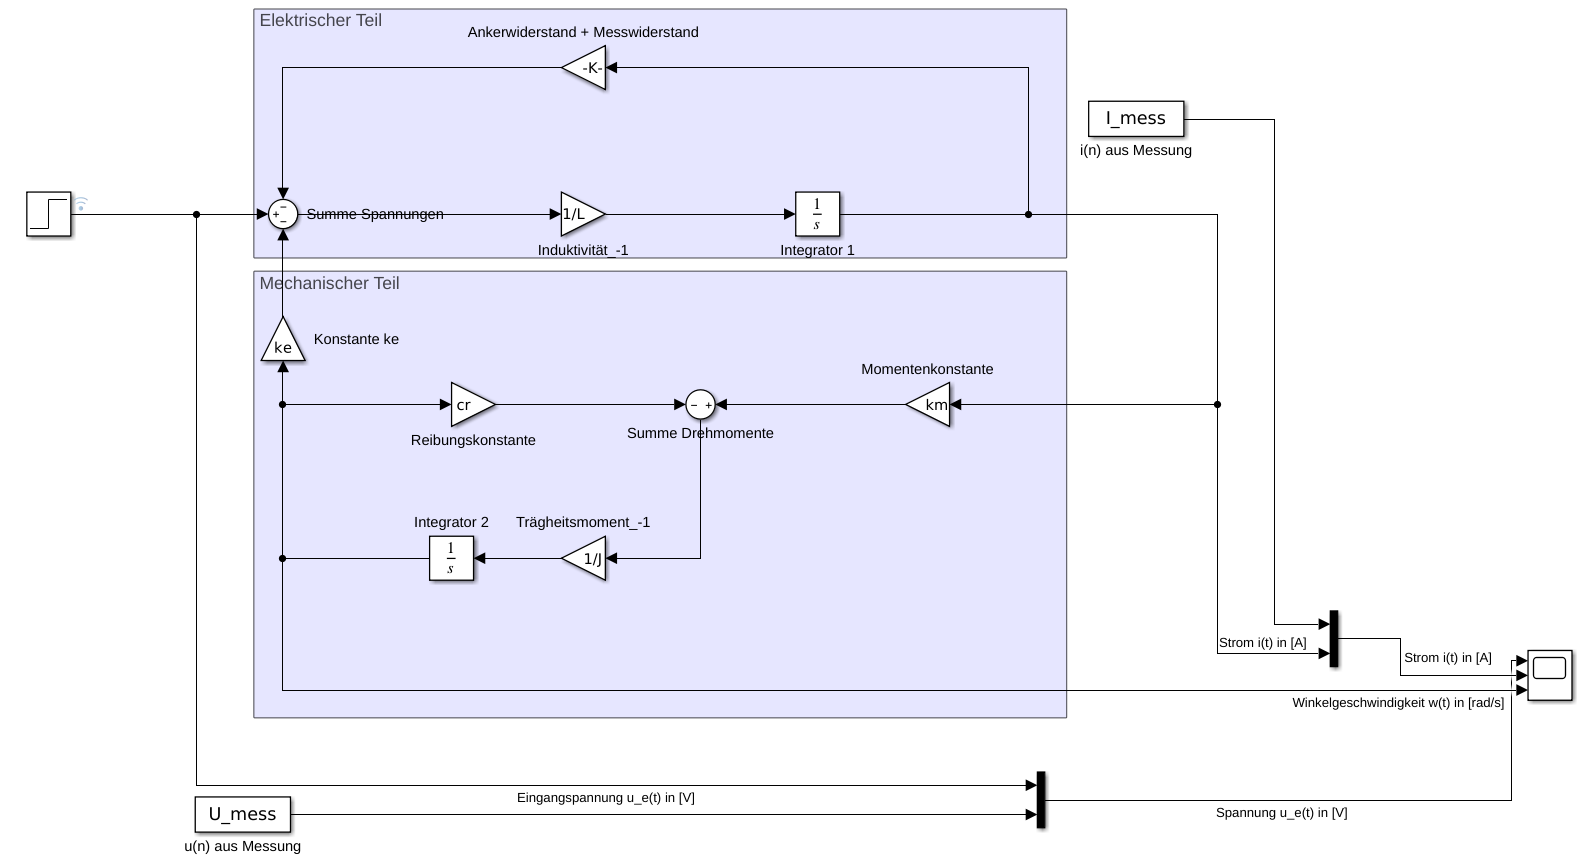
\includegraphics[width=1\textwidth]{sl_modell.png}
    \caption{Blockschaltbild in Simulink}
    \label{fig:Blockschaltbild}
\end{figure}

Als Eingang wurde ein Step-Block benutzt und als Ausgang ein Scope-Block.
Die erste DGL wurden im oberen Teil des Modell realisiert und beschreibt
den elektrischen Teil des Systems. Im unteren wird der mechanische Teil
des Motors modelliert der aus der zweiten DGL hervorgeht.\\

Die schon ermittelten Konstanten des Systems wurden in einem Matlab-File
abgespeichert und werden über dieses auch aufgerufen. Auch die Daten der
Messung des Spungs und der Sprungantwort sind hier zufinden.\\

Um den gemessenen Spung und die Sprungantwort in Simulink anzuzeigen wurde der Block
"From Workspace" benutzt der jeweils den Zeit-Spannungs-Vektor und den Zeit-
Spannungs-Vektor lädt.\\

Der Spung aus dem Modell wurden dem Sprung aus der Messung mit folgenden
Parameter angepasst.\\

\begin{figure}[H]
    \centering    
    \begin{tabular}[h]{l| r}
        Steptime & 0.048s \\
        \hline
        Final Value & 8.2V \\
        \hline
        Sampletime & 0.001s \\
    \end{tabular}
    \caption{Parameter Step Block}
\end{figure}
    

Um das Trägheitsmoment $J$ zu bestimmen, wurde dann $J$ auf den Initialwert
von $10^{-3}\mathrm{Kg \cdot m^2}$ gesetzt. Dieser stammt aus dem Datenblatt
des DCX10L aus der Vorlesung.

Danach haben wir das System für 30 Sekunden simuliert und erhielten folgendes
Ergebnis.

\begin{figure}[H]
    \centering
    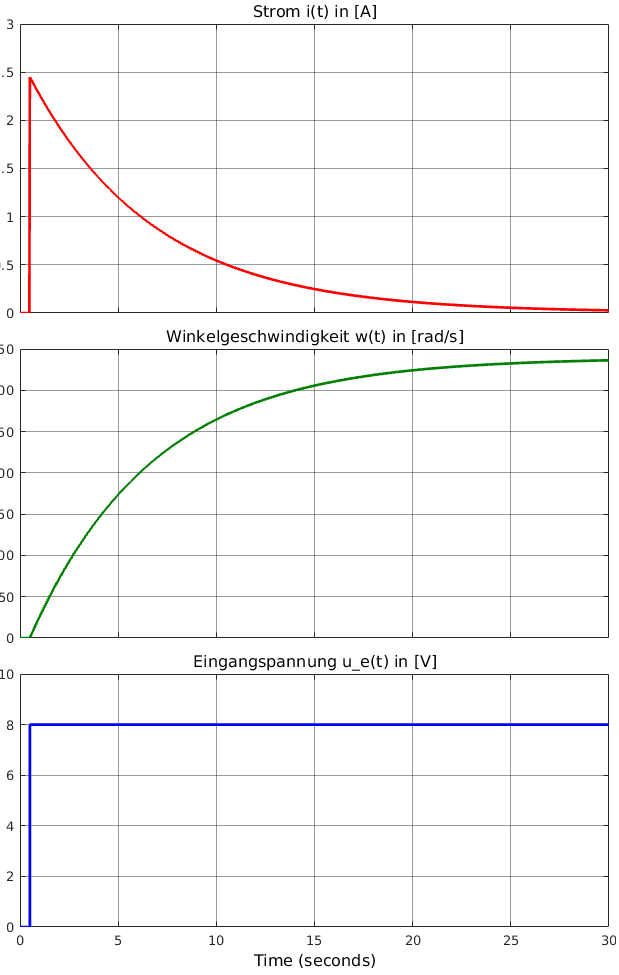
\includegraphics[width=0.75\textwidth]{data_modell.png}
    \caption{Simulation 1}
    \label{fig:Simulation 1}
\end{figure}

Wir haben dann durch manuelles iteratives Anpassen den Wert des Trägheitsmoments
so bestimmt, dass die Funktion des Modells mit den Messdaten übereinstimmt. 

\begin{equation} \label{eq311}
    \begin{split}
        J \simeq 5 \mathrm{\mu Kg \cdot m^2}
    \end{split}
\end{equation}

Anschließend simulierten wir in der Zeit der gegebenen Messdaten  $\Delta T= 0.6s$.
Daraus ergab sich folgendes Ergebnis.

\begin{figure}[H]
    \centering
    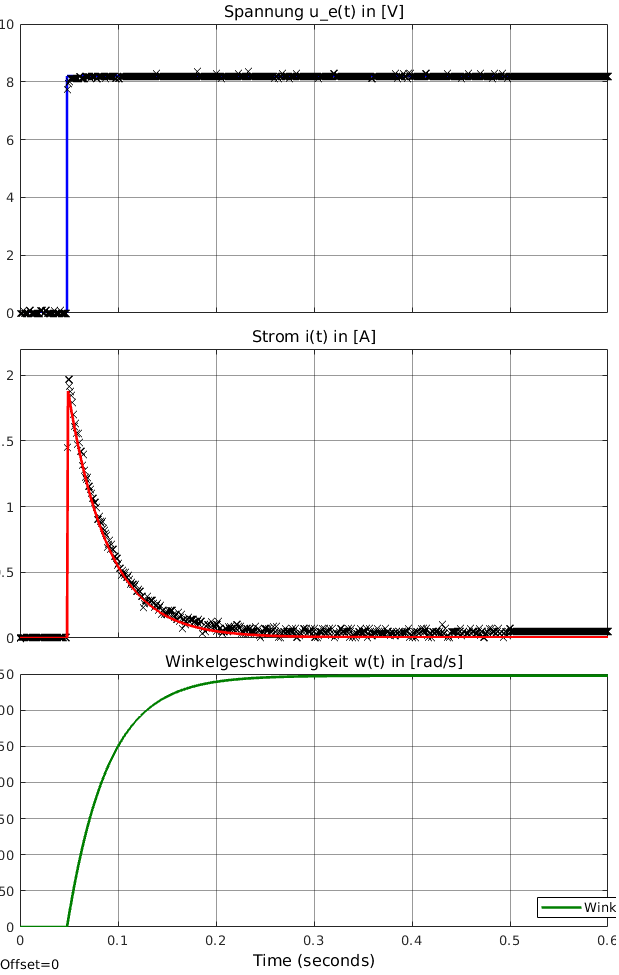
\includegraphics[width=0.75\textwidth]{data_modell_final.png}
    \caption{Simulation 2}
    \label{fig:Simulation 2}
\end{figure}
\subsection{Diskussion und Zusammenfassung}

Der exponentiell fallende Stromverlauf ist ein normales Verhalten des Anlaufstroms eines
Motors. Dies ist daher zu erklären, dass die Schwungmasse an der Welle des Motors aus
der Ruhelage erst auf Nenndrehzahl gebracht werden muss. Dafür ist im Anschaltmoment
eine große Energie nötig, welche über den erhöhten Strom zugeführt wird.\\

Die errechneten Funktionen unseres Modells stimmen nahezu vollständig mit den gemessenen
Daten überein. Sie liegen unter einer maximalen Abweichung von 5\%. Dieses gute Ergebnis
ist auf ein ausreichend gutes Modell und valide Messdaten zurückzuführen.\\
\subsection{Anhang}

\subsubsection{Aufgabenbeschreibung}
\begin{figure}[H]
    \centering
    \includegraphics[page=7, width=0.8\textwidth]{../Aufgabenstellung.pdf}
    %\caption{caption}
    \label{fig:Aufgabenstellung Labor 3}
\end{figure}


\subsubsection{Matlab Code}
\lstinputlisting[language=Matlab]{matlab/as_labor03_const_u_motor_dc.m}

%\subsubsection{Messwerte}

\end{document}
